\section{Ristrutturazione del Modello Concettuale}

Prima di poter passare allo schema logico è necessario ristrutturare il diagramma delle classi per semplificare la traduzione in schema logico, ottimizzare il progetto, eliminare le generalizzazioni, eliminare gli attributi multivalore, eliminare gli attributi strutturati, accorpare o partizionare le entità figlie e scegliere gli identifiatori delle nostre entità .\\


\subsection{Analisi delle Ridondanze}

Una ridondanza è un dato che è già presente nella base di dati o può essere derivato da altri dati. 

Nel modello concettuale originale non vi sono ridondanze; L'unico attributo derivato è 'Numero Afferenti' all'interno dell'entità Laboratorio. 
Questo attributo serve ad identificare quanti sono gli afferenti di un dato laboratorio ed è semplice ricavarlo attraverso il conteggio delle occorrenze fra il Laboratorio e gli Impiegati che vi afferiscono; Siccome i Laboratori sono gestiti da Progetti, per conoscere quanti sono gli Impiegati che lavorano ad un progetto bisognerebbe,senza questo attributo, passare per il conteggio delle varie occorrenze dei laboratori che lavorano al progetto, ciò viene semplificato inserendo l'attributo derivato in questione. 


\subsection{Analisi delle Generalizzazioni}
La specializzazione è il processo di determinazione di sottoclassi per una data entità. La generalizzazione è il suo concetto complementare.
Nel modello concettuale vi sono due specializzazioni diverse per la classe Impiegato.\newline
1.La specializzazione (totale, disgiunta) delle sotto-classi Junior, Middle e Senior che risolviamo accorpando queste classi figlie in quella padre Impiegato, inserendo un nuovo attributo 'tipo impiegato'.\newline
2.La specializzazione (parziale) della sotto-classe Dirigente che modelliamo accorpandola all'entità genitore, esprimendola invece come una singola flag booleana ' dirigente ';

\subsection{Eliminazione degli attributi Multivalore o Composti}
Un attributo è multivalore se può essere associato ad un numero variabile di valori dello stesso dominio. Un attributo è composto se può essere suddiviso in sottoparti ognuna dotata di dominio.

Nel modello concettuale non sono presenti attributi multivalore o composti.

\subsection{Analisi di Entità e Associazioni}
Non si è ritenuto necessario scomporre o accorpare entità.\\

\subsection{Scelta degli Identificatori Primari}

Un identificatore o chiave minimale è un insieme di attributi che individuano univocamente un'entità. È possibile che un'entità sia dotata di molteplici identificatori, fra i quali ne sceglieremo uno principale che agirà da chiave primaria.

\begin{itemize}
    \item \textbf{Impiegato}: fra le chiavi candidate Codice Fiscale e Matricola è stato scelta come chiave primaria Matricola in quanto più breve e indica naturalmente l'identificativo di ogni Impiegato.

    \item \textbf{Laboratorio}: si è deciso d'introdurre l'identificativo IdLab in quanto dai requisiti non si evince un attributo che identifica univocamente un laboratorio.

    \item \textbf{Progetto}: dalla traccia sono specificate due chiavi candidate precise : il CUP (codice univoco progetto) e il nome del progetto in quanto unico nel sistema. Si è preferito scegliere come chiave primaria il CUP.
    
    \item \textbf{Storico}: esso è un entità debole e, in quanto tale, non ha un attributo che identifica gli scatti di carriera poiché quest'ultimi non hanno motivo di esistere se non vi è un Impiegato a compierli; Comunque si decide come chiave parziale il nuovo ruolo e la data scatto.
\end{itemize} 

\newpage
\subsection{Diagramma Ristrutturato (UML)}
Dopo aver ristrutturato il Class Diagram come descritto precedentemente, possiamo produrre il seguente schema concettuale ristrutturato espresso mediante diagramma UML:

\begin{figure}[h!]

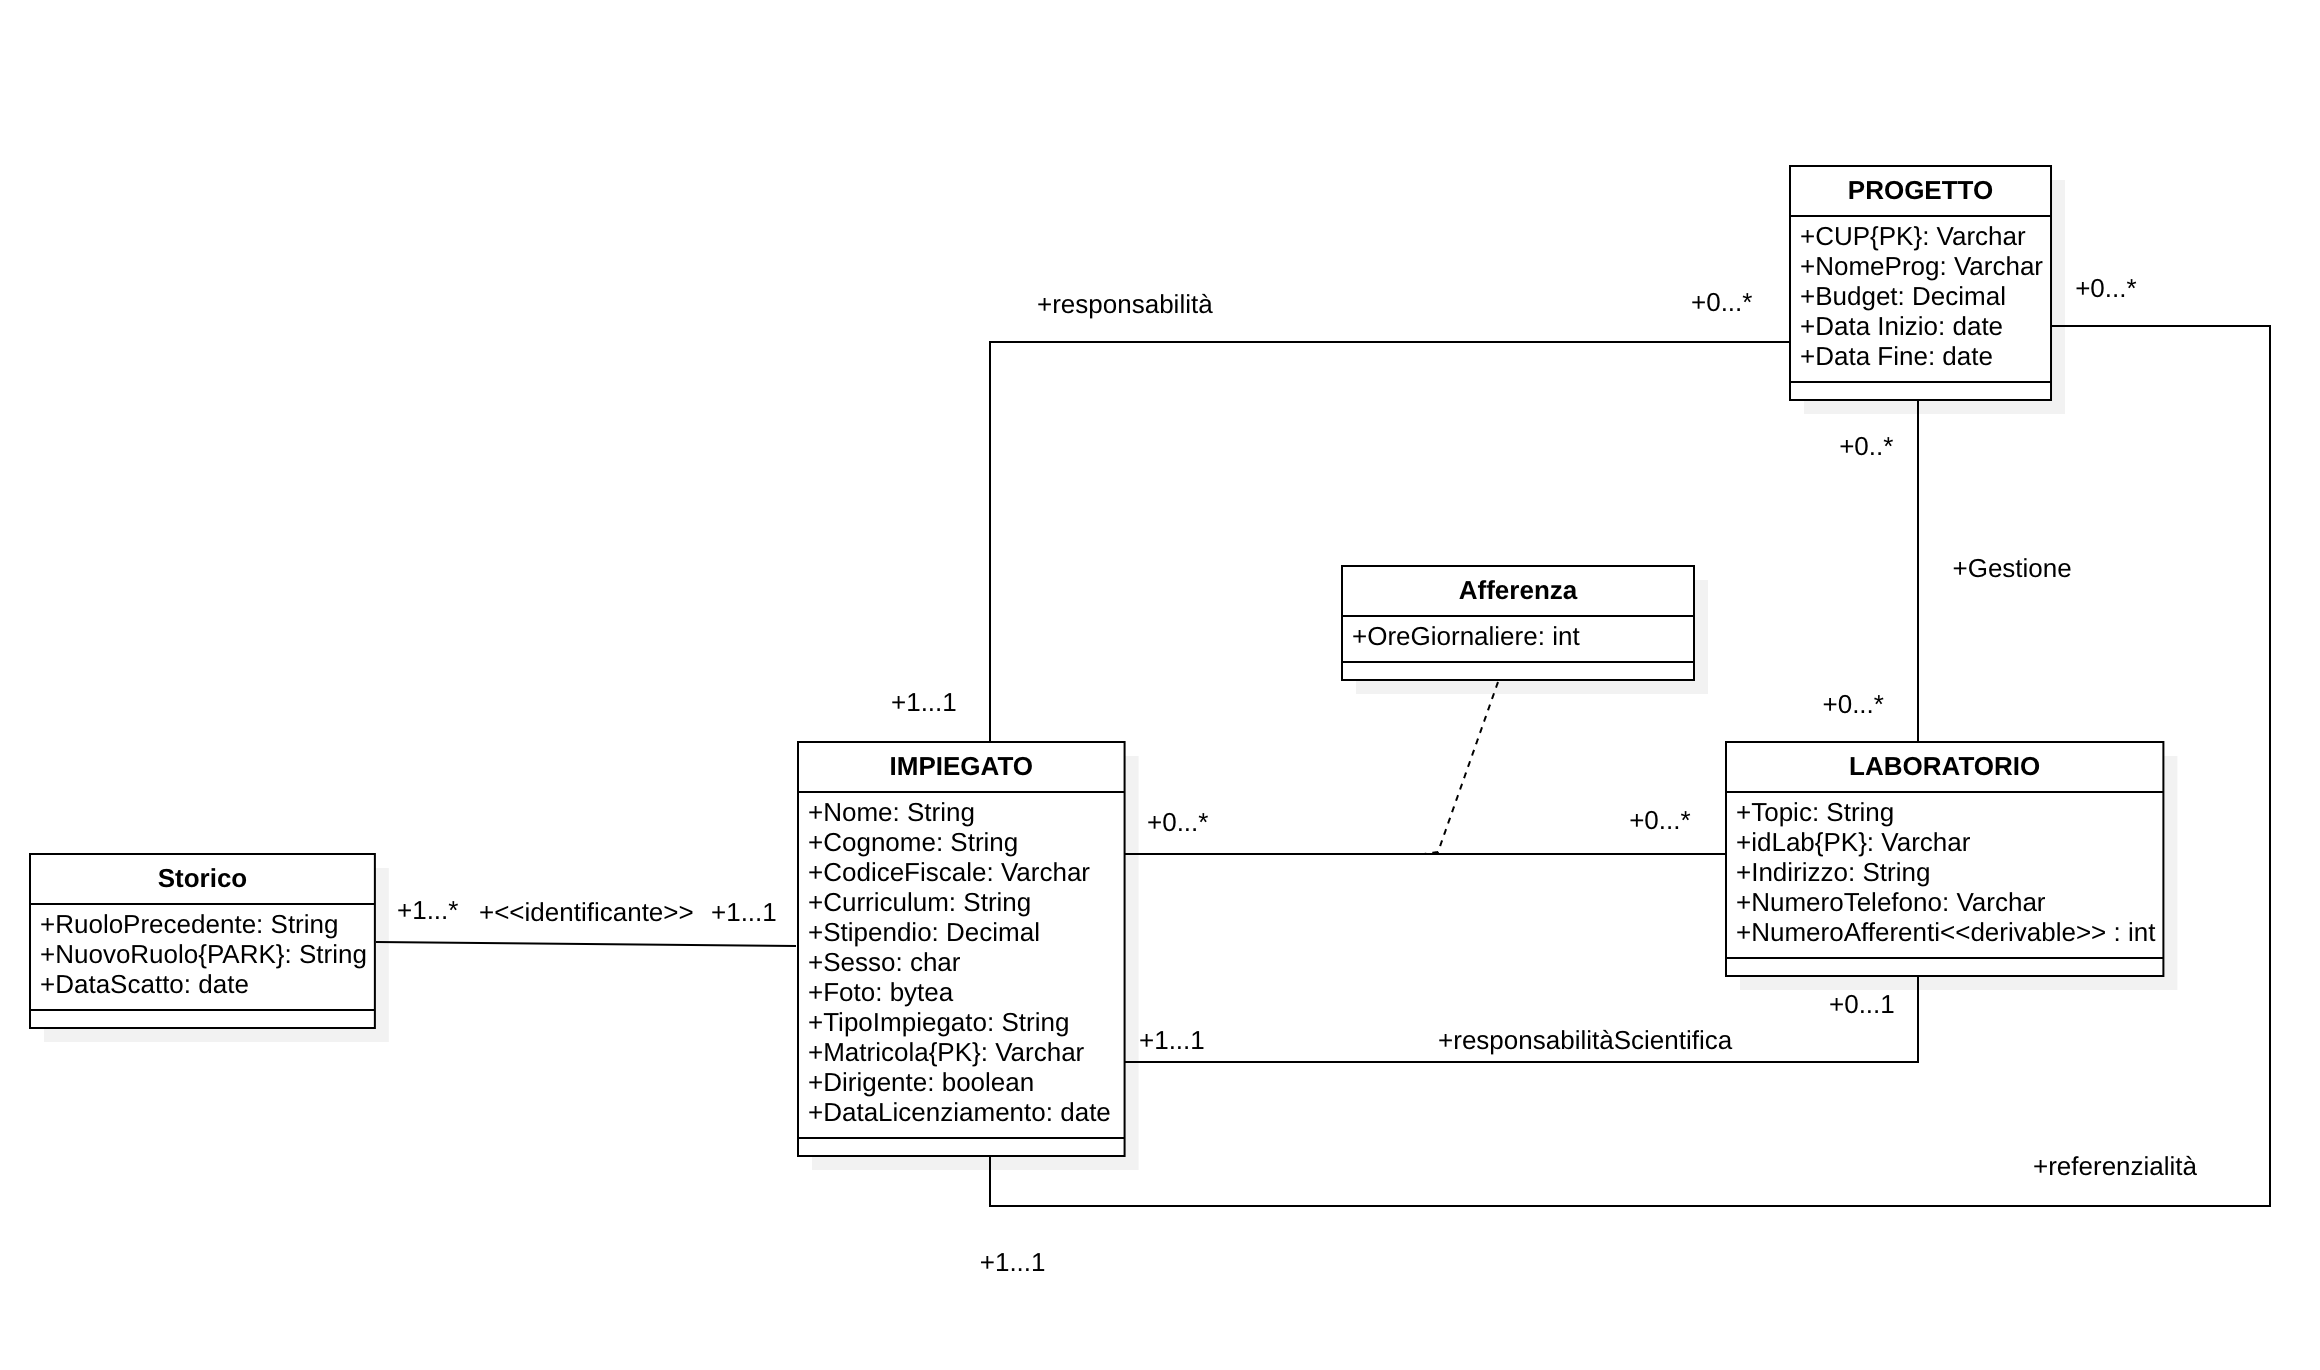
\includegraphics[width=\textwidth]{images/CONCETTUALE_RISTRUTTURATO.png}
\end{figure}

\newpage

\subsection{Diagramma Ristrutturato (ER)}
Ulteriore notazione per poter esprimere lo schema ristrutturato è il seguente l'ER :

\begin{figure}[h!]

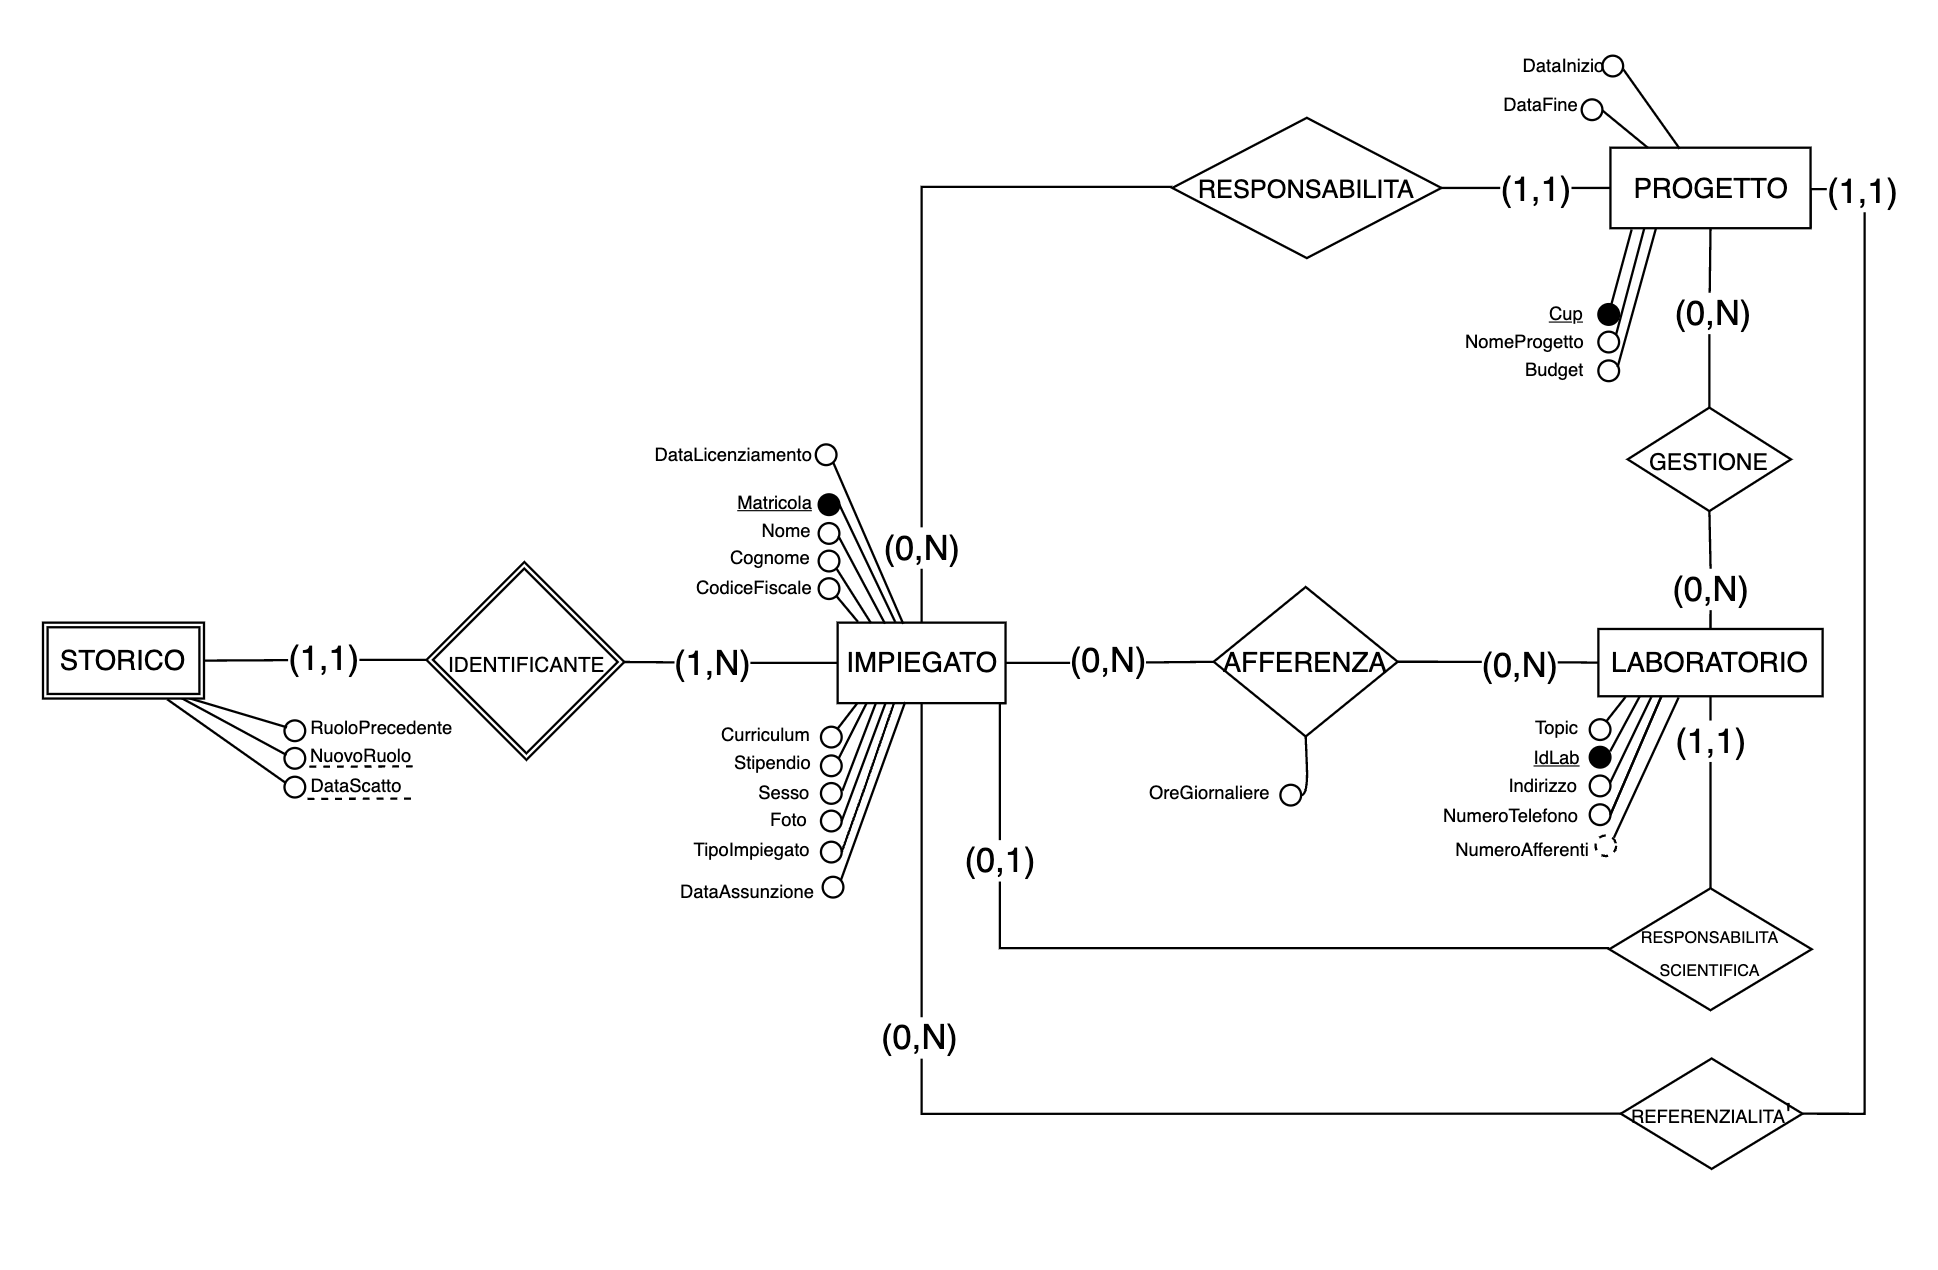
\includegraphics[width=\textwidth]{images/ER_RISTRUTTURATO.png}
\end{figure}